%%% LaTeX Template: Article/Thesis/etc. with colored headings and special fonts
%%%
%%% Source: http://www.howtotex.com/
%%% Feel free to distribute this template, but please keep to referral to http://www.howtotex.com/ here.
%%% February 2011
%%%
%%% Last updated September 2021 by CDM

%%%  Preamble
\documentclass[11pt,letterpaper]{article}
\usepackage[margin=1.0in]{geometry}
\usepackage[T1]{fontenc}
\usepackage[bitstream-charter]{mathdesign}
\usepackage[latin1]{inputenc}					
\usepackage{amsmath}						
\usepackage{xcolor}
\usepackage{cite}
\usepackage{hyphenat}
\usepackage{graphicx}
\usepackage{float}
\usepackage{subfigure}
\usepackage{sectsty}
\usepackage[compact]{titlesec} 
\usepackage[tablegrid]{vhistory}
\allsectionsfont{\color{accentcolor}\scshape\selectfont}

%%% Definitions
\definecolor{accentcolor}{rgb}{0.0,0.0,0.5} 
\newcommand{\teamname}{Team Name}
\newcommand{\productname}{Product Name}
\newcommand{\coursename}{CSE 4316: Senior Design I}
\newcommand{\semester}{Fall 2021}
\newcommand{\docname}{Project Charter}
\newcommand{\department}{Department of Computer Science \& Engineering}
\newcommand{\university}{The University of Texas at Arlington}
\newcommand{\authors}{Alan Turing \\ Grace Hopper \\ John Von Neumann \\ Ada Lovelace \\ Charles Babbage}

%%% Headers and footers
\usepackage{fancyhdr}
	\pagestyle{fancy}						% Enabling the custom headers/footers
\usepackage{lastpage}	
	% Header (empty)
	\lhead{}
	\chead{}
	\rhead{}
	% Footer
	\lfoot{\footnotesize \teamname \ - \semester}
	\cfoot{}
	\rfoot{\footnotesize page \thepage\ of \pageref{LastPage}}	% "Page 1 of 2"
	\renewcommand{\headrulewidth}{0.0pt}
	\renewcommand{\footrulewidth}{0.4pt}

%%% Change the abstract environment
\usepackage[runin]{abstract}			% runin option for a run-in title
%\setlength\absleftindent{30pt}			% left margin
%\setlength\absrightindent{30pt}		% right margin
\abslabeldelim{\quad}	
\setlength{\abstitleskip}{-10pt}
\renewcommand{\abstractname}{}
\renewcommand{\abstracttextfont}{\color{accentcolor} \small \slshape}	% slanted text

%%% Start of the document
\begin{document}

%%% Cover sheet
{\centering \huge \color{accentcolor} \sc \textbf{\department \\ \university} \par}
\vspace{1 in}
{\centering \huge \color{accentcolor} \sc \textbf{\docname \\ \coursename \\ \semester} \par}
\vspace{0.5 in}
\begin{figure}[h!]
	\centering
   	
\includegraphics[width=0.60\textwidth]{images/test_image}
\end{figure}
\vspace{0.5 in}
{\centering \huge \color{accentcolor} \sc \textbf{\teamname \\ \productname} \par}
\vspace{0.5 in}
{\centering \large \sc \textbf{\authors} \par}
\newpage


%\vspace{1 in}
%\centerline{January 13th, 2012}
%\newpage

%%% Revision History
\begin{versionhistory}
  	\vhEntry{0.1}{10.01.2021}{GH}{document creation}
  	\vhEntry{0.2}{10.05.2021}{AT|GH}{complete draft}
  	\vhEntry{0.3}{10.12.2021}{AT|GH}{release candidate 1}
  	\vhEntry{1.0}{10.20.2021}{AT|GH|CB}{official release}
  	\vhEntry{1.1}{10.31.2021}{AL}{added customer change requests}
\end{versionhistory}
\newpage

%%% Table of contents
\tableofcontents
\newpage

%%% List of figures and tables (optional)
\listoffigures
%\listoftables
\newpage
\setcounter{table}{0}

%%% Executive summary sections
\section{Problem Statement}
The problem statement defines the "Why" of the project. This is the higher purpose, or the reason for the project's existence. This section should avoid mentioning implementation details, and focus more on what the current problem is and what would be gained if the problem were to be solved. In short, the is the reason that you are going to be working on something, not the method(s) that you will be employing.
\section{Methodology}
The objective of this project is to enhance the capabilities of an RV8 robot work cell by integrating various component
, including an end-effector (gripper), a laser safety scanner, emergency stop (E-stop) switches, a MELSEC PLC controller
, a host PC, and a linear rail. The integration aims to facilitate advanced control applications such as pick and place,
palletizing, and depalletizing while ensuring compliance with safety standards.
Currently, the work cell lacks the necessary components and configurations to operate efficiently and safely in a
dynamic environment. The project will focus on developing a robust control application that not only enables the desired
robotic operations but also incorporates critical safety features, including safety cutoffs and direct entry presence
detection. This integration is vital to minimize operational risks and enhance productivity within the work cell.By
addressing these goals, the project aims to transform the RV8 robot work cell into a highly capable, safe, and efficient
automated solution for industrial applications
\section{Value Proposition}
To address the challenges of smart manufacturing, a structured methodology will be implemented, starting with a comprehensive assessment of current manufacturing processes, technologies, and workforce capabilities. This phase will involve gap analysis and technology audits to identify integration needs. Following this, a detailed technology roadmap will be developed to facilitate the seamless integration of advanced technologies with legacy systems, supported by pilot projects for real-world validation.

Simultaneously, a targeted workforce development program will be designed to close skill gaps, focusing on training in new technologies and cybersecurity best practices. A robust cybersecurity framework will be established through risk assessments and regular audits. Finally, key performance indicators (KPIs) will be defined to measure success, alongside a feedback mechanism for continuous improvement. This systematic approach aims to enable organizations to  transition effectively to smart manufacturing, enhancing efficiency and competitiveness in the market.
\section{Development Milestones}
The following is a list of completion dates for all major documents, demonstrations, and associated deadlines:
\begin{itemize}
  \item Project Charter Final Draft             - September 30, 2024
  \item System Requirements Specification       - October   21, 2024
  \item Architectural Design Specification      - November   4, 2024
  \item Demonstration of MELSEC PLC Programming - November,     2024
  \item Demonstration of E-Stop Switch          - November,     2024
  \item Demonstration of Laser Safety Scanner   - December,     2024
  \item Demonstration of Linear Rail Movement   - January,      2024
  \item Demonstration of Gripper Configuration  - February,     2024
  \item Demonstration of Basic Stacking         - March,        2024
  \item Demonstration of Palletizing Algorithm  - March,        2024
  \item CoE Innovation Day poster presentation  - April     16, 2024
  \item Final Project Demonstration             - April,        2024    
  \item Final Project Submission                - May        1, 2024
\end{itemize}


\newpage

%%% Remaining project charter sections
\section{Background}
%% It is just an empty TeX file.
%% Write your code here.
Historically, interactions between humans and industrial robots have been major safety concerns. Early factory environments did not focus on human safety in these conditions. This often resulted in strict separation between workers and machines, with physical barriers and lock-out protocols put in place to prevent accident or injury. These set-ups created restricted zones around machinery, and created hazardous conditions whenever human interaction or intervention with the equipment was necessary. Human intervention with a palletizing robot is often necessary for troubleshooting errors in the production line, such as a misplaced or trapped box on the conveyor belt. In these situations, workers must enter the robot’s operating zone to correct the issue, which is dangerous in traditional set-ups.

In a factory palletization setting, the UR20 Cobot offers a safety advantage compared to traditional heavy machinery. Whereas conventional automated systems which often require physical barriers or guarded zones to protect workers from potential harm, the UR20 is specifically engineered for safe human interaction. Its integrated sensors detect physical touch and respond to any notable resistance by stopping movement immediately. This built-in responsiveness drastically reduces the risk of accidents, even when the cobot is performing tasks that involve lifting heavy payloads. This makes it no longer necessary to guard the operating area with restricted zones or physical barriers, allowing for more efficient operation and greater worker safety.

Our implementation of the UR20 Cobot includes proximity detection and camera systems capable of recognizing human presence. These technologies allow the cobot to anticipate and respond to the presence of nearby workers, reducing the possibility of workplace accidents.


\section{Related Work}

Automation is an emerging state-of-the-art technology in manufacturing and logistics, advancing signinficantly year after year. These solutions are available in various forms, including academic research, commercial use, and prototypes. There are several commercial solutions to optimizing work efficiency with automated robots, each with their own strengths and weaknesses. One of the large commercially available solutions is Robotiq's robotic palletizing solution, that can be installed in days and resolve production instability \cite{Robotiq2024}. Despite the advantages, solutions such as these are very costly where the palletizing application of the RV8 would cut costs.

Robotic palletizing is also a popular topic in academic research, focusing on the algorithms for object recognition, position control, and planning \cite{Xu2022}. Additionally power consumption plays a large role in the cost of operation, and is a field that is researched to reduce operating power consumption \cite{Deng2022}. Furthermore, while many solutions claim to be easily deployable they often require substantial training on how to operate the system. The RV8 palletizing application will tackle this problem with the process and setup being documented. Industrial solutions also exist to face growing demands to improve efficiency, utilizing industrial wireless sensor networks for rapid deployment and flexibility \cite{Gungor2009}. Lastly, a major factor in the efficiency of the palletization application is the vision of the robot. The time for recognition of an object and its dimenisons are incredibly important for selection and placement \cite{Abdullah2022}. Our RV8 robot will feature a gripper and vision system to efficiently detect objects and determine the best fit location for it.

\section{System Overview}
The overall structure of the software system is designed to seamlessly support the palletizing tasks of the UR20 robot arm system. This layered design enables modular functionality, enhancing system adapability and ensuring each layer performs a unique function while simultaneously providing crucial information to the main PLC layer which manages data distribution. As the central interface, the PLC efficiently processes the flow of sata from each subsystem layer, allowing for smooth system integration and effective coordination across all layers. This architecture promotes reliable, dynamic operation, optimizing the UR20's performance in real-time palletizing tasks.
\begin{figure}[h!]
	\centering
 	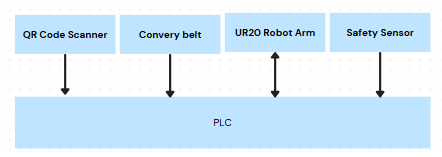
\includegraphics[width=0.60\textwidth]{images/layers}
 \caption{UR20 Architectural design diagram}
\end{figure}

\subsection{Layer 1: PLC Description}
The PLC will process most of the data through its peripherals, as seen in Figure 1. It is the primary interface between the different layers of the project. The built-in PLC will be configured with URScript, a Python-based scripting language in which vital functions will reside, such as the input function, the box offset algorithm, and finally, a position algorithm. The data flow will start with the input given by the QR code scanner or the safety sensor, and the input functions will follow these two data paths. First being, an input given by the QR code scanner will pass through the input function, which will then call the box offset algorithm to determine where the box is in 3D space given the location info from the QR code, which will go to the position algorithm which will determine the motion necessary for the UR20 to satisfy this request. The safety algorithm will give the second path, which will trigger the input function and call the position algorithm to safely slow down the speed at which the UR20 is palletizing to create a safe work area for a cooperative application.

\subsection{Layer 2: Safety Sensor}
The Safety Sensor will determine if a human is in the area of the UR20 arm. If so, it will reduce the speed of the UR20 in order to create a safe work environment. This will be achieved with the use of a camera that will process the data in real-time with the use of computer vision, which will send a signal to the PLC which in turn will send a signal to the UR20 movement subsystem in order to maintain a safe speed for collaborative work.

\subsection{Layer 3: UR20 Robot Arm}
UR20 Arm consists of a vacuum gripper, the gripper controller, and the movement of the arm. The arm is the physical output of the software that resides in the PLC layer. Additionally, it contains a gripper grab/release controller (the controller for the air compressor), which will be turned on or off when needed to hold or drop a box. The commands given by the PLC will determine the position and orientation needed for the UR20 to place the box correctly.

\subsection{Layer 4: QR Code Scanner}
Implementing QR code technology will enhance the automation and accuracy of arranging boxes on a pallet. When a box arrives on the conveyor belt, a QR code scanner positioned above the belt reads the QR code on the box. This QR code contains data such as box size, weight, and any other relevant handling instructions. Once scanned, the data is immediately sent to a Programmable Logic Controller (PLC) on a Universal Robots UR20 robotic arm system, which is responsible for arranging the boxes on the pallet.

\subsection{Layer 5: Conveyor Belt}
The conveyor belt system moves over pulleys driven by a motor. As the motor rotates, it propels the belt forward, allowing items placed on the belt to be conveyed along its length. The belt's speed can be adjusted to control the pace of movement. However, for this implementation, it will have two states: on or off. At the end of the conveyor belt, there will be a guide to reorient the boxes and a bracket in which the QR code scanner will be placed.
\section{Roles \& Responsibilities}
Who are the stakeholders of the project? Who will be the point of contact from the sponsor or customer side? Who are the team members, and what will be their areas of responsibility? Will your team maintain the product owner and scrum master for the whole project, or will that role change periodically? This section should occupy 1/2 - 1 full page.
\section{Cost Proposal}
This proposal will be focusing on the UR20 Cobot, although the original design was for the Mitsubishi RV8 arm.

\subsection{Current \& Pending Support}
This project's funding currently consists of only the default \$800 funding from the CSE department. More funding may be provided with sufficient justification, but no other funding sources are currently known.

    Current total funds:
    \begin{itemize}
        \item \$800 Default Budget
    \end{itemize}

\subsection{Final Budget}
The final cost of our project as of April 2025 is listed here.
The UR20 Cobot has a provided safety scanner, wiring box, and conveyor belt. A gripper will need to be purchased or designed in order for it to perform a palletizing application.

The item that ended up being chosen was a custom-design suction-cup gripper using parts borrowed from the Senior Design labs and 3D printed materials. \$300 worth of suction cups were purchased before an unused, higher-quality alternative was found in the labs.  


This table records the cost of all acquired items for the project.
\begin{table}[H]
\centering
    \caption{Budget itemization}
    \begin{tabular}{|l|l|}
        \hline
        \textbf{Item} & \textbf{Price} \\ \hline
        End effector and components & \$300+ \\ \hline
        Vacuum pump  and components & \$0 \\ \hline
        Mounting bracket & \$0\\ \hline
        Feeder belt & \$0 \\ \hline
        Photoeye detector & \$30 \\ \hline
        Miscellaneous small parts (screws, shaft collars, etc) & \$100 \\ \hline
        Raspberry Pi and camera & \$0 \\ \hline
        Boxes and pallet & \$0 \\ \hline
    \end{tabular}
\end{table}

\subsection{Preliminary Budget}
 The original options considered at the creation of this document are listed here.

\begin{itemize}
    \item A conveyor belt will likely be necessary for simulation of a real-world factory palletizing environment's margin of error.
    \item A vacuum generator will be needed, either included in the gripper or acquired separately.
    \item For palletizing, it is likely that a suction grip will be the most effective. However, those grips can be extremely expensive, likely coming in at a minimum of \$2000 unless used parts can be found. This is due to the necessity of a vacuum generator attached before the actual gripper in order to provide it power.
    \item Some more light-weight grippers have been designed for other robots such as MyCobot, and may be translatable to our robot. This would cost only \$400, and should be explored by reaching out to those manufacturers for questions.
    \item We could also, as the most time-consuming option, take inspiration from existing designs of vacuum pumps or end effectors and design one of the components, using the remaining money to invest in the other component. 
\end{itemize}


This table assumes we will purchase the cheapest versions of the above options instead of making them ourselves.
\begin{table}[H]
\centering
    \caption{Budget planning}
    \begin{tabular}{|l|l|}
        \hline
        \textbf{Item} & \textbf{Price} \\ \hline
        End effector and components & \$400+ \\ \hline
        Vacuum pump  and components & \$200+ \\ \hline
        Mounting bracket & \$100\\ \hline
        Feeder belt & \$100 \\ \hline
    \end{tabular}
\end{table}

\section{Facilities \& Equipment}
%% It is just an empty TeX file.
%% Write your code here.
The RV8 Robot Work Cell project is located in ERB 335, a designated laboratory area. The lab area includes the appropriate electrical infrastructure accommodating the power requirements of the RV8 robot. As for Safety measures the lab provides an access only secure work environment for the operator and equipment.


As for equipment, the lab in ERB 335 contains most components. The RV8 Robot itself has the capability of performing various tasks with precision, speed, and versatility. The RV8 will equip the MELSEC and PLC to provide a reliable and precise system to control and program the robot. The robot will also be able to move along a linear rail enhancing versatility. A laser will also be integrated in order to enhance safety of the operator around the arm. Other components like the gripper will likely need to purchased and will allow the RV8 robot to perform tasks such as palletizing 

\section{Assumptions}
\begin{itemize}
  \item The gripper suitable for pallaetizing will be purchased/designed by the 3rd sprint cycle 
  \item There will be sufficient space in ERB 335 for the robot's palletizing application
  \item The Engineering Research Building will provide stable internet connectivity and sufficient power 
  \item The exisiting saftety scanner and PLC setup is fully functional without significant reconfiguration following the integration of a gripper
  \item All necessary toools and equipment will be provided and readily available in ERB 335
\end{itemize}
\section{Constraints}
Constraints are limitations imposed on the project, such as the limitation of cost, schedule, or resources, and you have to work within the boundaries restricted by these constraints. All projects have constraints, which are defined and identified at the beginning of the project.

Constraints are outside of your control. They are imposed upon you by your client, organization, government regulations, availability of resources, etc. Occasionally, identified constraints turn out to be false. This is often beneficial to the development team, since it removes items that could potentially affect progress.

This section should contain a list of at least 5 of the most critical constraints related to your project. For example:

The following list contains key constraints related to the implementation and testing of the project.

\begin{itemize}
  \item Final prototype demonstration must be completed by May 1st, 20XX
  \item The customer will provide no more than two maintenance personnel to assist in on-site installation
  \item Customer installation site will only be accessible by development team during normal business hours
  \item Total development costs must not exceed \$800
  \item All data obtained from customer site must be reviewed and approved for release by the Information Security Office prior to being copied to any internet connected storage medium
\end{itemize}

\section{Risks}
\begin{table}[H]
    \resizebox{\textwidth}{!}{
    \begin{tabular}{|l|l|l|l|}
    \hline
    \textbf{Risk description} & \textbf{Probability} & \textbf{Loss (days)} & \textbf{Exposure (days)} \\ \hline
    Shipping delay on gripper parts                    & 0.50 & 30 & 15    \\ \hline
    Unable to find compatible gripper for product task & 0.05 & 40 & 2     \\ \hline
    Issues with hardware or gripper behavior           & 0.20 & 7  & 1.4    \\ \hline
    Difficulty with PLC setup or connecting to host PC & 0.20 & 5  & 1     \\ \hline
    Delay due to member being ill                      & 0.05 & 5  & .25   \\ \hline
    \end{tabular}}
    \caption{Overview of highest exposure project risks} 
\end{table}
\section{Documentation \& Reporting}
%%% In this section, you will describe all of the various artifacts that you will generate and maintain during the project life cycle. Describe the purpose of each item below, how the content will be generated, where it will be stored, how often it will be updated, etc. Replace the default text for each section with your own description. Reword this paragraph as appropriate.

\subsection{Major Documentation Deliverables}
These deliverables are major grade components of the course. Completing these documents should generally be the sprint goal during the applicable sprint period. Refer to current and previous course syllabi and schedules to estimate the due dates of these items. Remove this explanatory paragraph from your draft, but leave the heading.

\subsubsection{Project Charter}
Describe how this document will be maintained and updated (how often, under what circumstances, etc.). When will the initial version be delivered? When will the final version be delivered?

\subsubsection{System Requirements Specification}
Describe how this document will be maintained and updated (how often, under what circumstances, etc.). When will the initial version be delivered? When will the final version be delivered?

\subsubsection{Architectural Design Specification}
Describe how this document will be maintained and updated (how often, under what circumstances, etc.). When will the initial version be delivered? When will the final version be delivered?

\subsubsection{Detailed Design Specification}
Describe how this document will be maintained and updated (how often, under what circumstances, etc.). When will the initial version be delivered? When will the final version be delivered?

\subsection{Recurring Sprint Items}
The following items will be documented and maintained during each individual sprint. As above, remove this paragraph from your draft, but leave the heading.

\subsubsection{Product Backlog}
How will items be added to the product backlog from the SRS? How will these items be prioritized? Who makes the decision (product owner, group vote, etc.)? What software will be used to maintain and share the product backlog with team members and stakeholders?

\subsubsection{Sprint Planning}
How will each sprint plan be planned? How many sprints will there be (you need to look at the schedules for this course and previous Senior Design II courses during the appropriate semesters to figure this out).

\subsubsection{Sprint Goal}
Who decides the sprint goal? How will you involve your customer in this process?

\subsubsection{Sprint Backlog}
Who decides which product backlog items make their way into the sprint backlog? How will the backlog be maintained (collaboration software, a "scrum board", etc.)?

\subsubsection{Task Breakdown}
How will individual tasks be assigned from the sprint backlog? Will it be up to each team member to voluntarily claim a task, or will it come from the product owner? How will time spent on tasks be documented?

\subsubsection{Sprint Burn Down Charts}
Who will be responsible for generating the burn down charts for each sprint? How will they be able to access the total amount of effort expended by each individual team member? What format will the burn down chart use (include an example burn down chart below).

\begin{figure}[h!]
    \centering
    
\includegraphics[width=0.5\textwidth]{images/test_image}
    \caption{Example sprint burn down chart}
\end{figure}

\subsubsection{Sprint Retrospective}
How will the sprint retrospective be handled as a team? When will this discussion happen after each sprint? What will be documented as a group and as individuals, and when will it be due?

\subsubsection{Individual Status Reports}
What sort of status will be reported by each individual member, and how often will it be reported? What key items will be contained in the report?

\subsubsection{Engineering Notebooks}
How often will the engineering notebook be updated, at a minimum, by each team member? What is the minimum amount of pages that will be completed for each interval, and how long will that interval be? How will the team keep each member accountable? Who will sign of as a "witness" for each ENB page?

\subsection{Closeout Materials}
The following materials, in addition to major documentation deliverables, will be provided to the customer upon project closeout. Remove this paragraph from your draft, but leave the heading.

\subsubsection{System Prototype}
What will be included in the final system prototype? How and when will this be demonstrated? Will there be a Prototype Acceptance Test (PAT) with your customer? Will anything be demonstrated off-site? If so, will there be a Field Acceptance Test (FAT)?

\subsubsection{Project Poster}
What will be included on the poster, what will be the final dimensions, and when will it be delivered?

\subsubsection{Web Page}
What will be included on the project web page? Will it be accessible to the public? When will this be delivered? Will it be updated throughout the project, or just provided at closeout (at a minimum, you need to provide a simple web page at the end).

\subsubsection{Demo Video}
What will be shown in the demo video(s)? Will you include a B-reel footage for future video cuts? Approximately how long will the video(s) be, and what topics will be covered?

\subsubsection{Source Code}
How will your source code be maintained? What version control system will you adopt? Will source code be provided to the customer, or binaries only? If source code is provided, how will it be turned over to the customer? Will the project be open sourced to the general public? If so, what are the license terms (GNU, GPL, MIT, etc.). Where will the license terms be listed (in each source file, in a single readme file, etc.).

\subsubsection{Source Code Documentation}
What documentation standards will be employed? Will you use tools to generate the documentation (Doxygen, Javadocs, etc.). In what format will the final documentation be provided (PDF, browsable HTML, etc.)?

\subsubsection{Hardware Schematics}
Will you be creating printed circuit boards (PCBs) or wiring components together? If so, list each applicable schematic and what sort of data it will contain (PCB layout, wiring diagram, etc.). If your project is purely software, omit this section.

\subsubsection{CAD files}
Will the project involve any mechanical design, such as 3D printed or laser-cut parts? If so, what software will you use to generate the files and what file formats will you provide in your closeout materials (STL, STEP, OBJ, etc.). If your project is purely software, omit this section.

\subsubsection{Installation Scripts}
How will the customer deploy software to new installations? Will you provide installation scripts, install programs, or any other tools to improve the process? Will there be multiple scripts provided (perhaps separate scripts for the graphical front end and back end server software)? 

\subsubsection{User Manual}
Will you customer need a printed or digital user manual? Will they need a setup video? Decide now what will be provided and discuss.

\newpage

%%% References
\bibliographystyle{plain}
\bibliographystyle{reference/IEEEtran_custom}
\bibliography{reference/refs}{}

\end{document}